\documentclass{article}

\usepackage[preprint]{project_440_550}

\usepackage[utf8]{inputenc}
\usepackage[T1]{fontenc}
\usepackage[USenglish]{babel}
\usepackage{csquotes}

\usepackage{booktabs}
\usepackage{amsmath}
\usepackage{microtype}
\usepackage{xcolor}
\usepackage{graphicx}
\usepackage{hyperref}
\usepackage{url}

\usepackage[style=authoryear,maxbibnames=30,natbib]{biblatex}
\addbibresource{refs.bib}
\renewbibmacro{in:}{}
\DeclareDelimFormat{nameyeardelim}{\addspace}
\DeclareNameAlias{sortname}{given-family}

\usepackage[capitalize,noabbrev]{cleveref}

\definecolor{goodgreen}{HTML}{1b7a3b}
\definecolor{badred}{HTML}{b22222}
\newcommand{\pos}[1]{\textcolor{goodgreen}{$+#1$}}
\newcommand{\neg}[1]{\textcolor{badred}{$-#1$}}


\title{Prompt Repetition Finetuning is All You Need. Prompt Repetition Finetuning is All You Need. }

\author{%
  Noah Marusenko\\
  \texttt{nmarusen@student.ubc.ca}
  \And
  Alain Zhiyanov\\
  \texttt{azhiyano@student.ubc.ca}
  \And
  Andrew Ahn\\
  \texttt{tahn01@student.ubc.ca}
}


\begin{document}
\maketitle


\begin{abstract}
\citet{leviathan2025} recently showed that simply repeating a prompt
before generation---feeding the model \texttt{prompt + prompt} instead
of \texttt{prompt}---improves the accuracy of non-reasoning language
models at inference time. We ask whether the same idea also helps during
fine-tuning. We LoRA fine-tune three instruction-tuned models
(Qwen2.5-1.5B, Mistral-7B, Qwen2.5-7B) on a 13.5k-example mixture of
ARC-Challenge, OpenBookQA, and GSM8K with doubled prompts, and evaluate
on seven benchmarks (three in the training mix, four held out). Training
on doubled prompts produces large in-distribution gains (up to $+17$
accuracy points on OpenBookQA for Qwen2.5-1.5B)---much larger than the
inference-time effect on its own. However, the gains transfer poorly to
held-out tasks, and for Mistral-7B the fine-tuned model collapses on
open-ended math generation (GSM8K drops from $7.9\%$ to $0.1\%$). We
conclude that prompt repetition is \emph{learnable}, but behaves more
like a cheap data-format trick than a universal improvement.
\end{abstract}


\section{Introduction}

Causal-attention language models process tokens strictly left-to-right,
so information early in the prompt cannot benefit from later context.
\citet{leviathan2025} observed that a one-line change mitigates some of
this asymmetry: repeat the entire prompt once before the model answers.
They report small but consistent improvements across many
non-reasoning models with no training and essentially no extra compute.

We ask the natural follow-up: \emph{if doubling the prompt helps at
inference, does it also help during training?} Concretely, does
fine-tuning on \texttt{prompt + prompt $\to$ answer} examples beat
both the vanilla base model and the vanilla model with inference-time
doubled prompts? There are two reasons to expect that it might.
Inference-time repetition creates a train/test distribution mismatch
that fine-tuning closes, and repeatedly training on doubled prompts
could plausibly encourage the model to internalize more
context-complete attention patterns.

\paragraph{Contributions.} We LoRA fine-tune three instruction-tuned
models (Qwen2.5-1.5B, Mistral-7B, Qwen2.5-7B) on the same doubled-prompt
data, and evaluate each under three conditions---vanilla+single,
vanilla+double, fine-tuned+double---on seven benchmarks, four of them
strictly held out. We find that (i) inference-time double prompting
reproduces \citet{leviathan2025}'s small gains on the two 7B models but
not on the 1.5B model; (ii) training on doubled prompts gives much
larger in-distribution gains than inference-time repetition; but (iii)
those gains largely do not transfer, and can catastrophically damage
open-ended generation when the training mix is biased toward short
multiple-choice answers.


\section{Related work}

Our work is a direct training-time follow-up to \citet{leviathan2025},
who study prompt repetition only at inference. More broadly, prompt
repetition is one of many techniques that have been promoted from
inference tricks into training signals; our question is whether this
particular one is worth promoting.
We fine-tune with LoRA \citep{hu2022lora}, which makes it cheap to repeat
the same experiment across multiple base models.


\section{Method}

\paragraph{Training objective.} Let $p$ be a prompt (system message plus
question, in the base model's chat template) and $y$ the gold answer.
Standard instruction tuning minimizes $-\log p_\theta(y \mid p)$; we
instead minimize
\[
  \mathcal{L}_{\text{double}}(\theta)
  = -\log p_\theta\bigl(y \,\big|\, p \,\Vert\, p\bigr),
\]
where $p \Vert p$ concatenates two copies of the question block with a
blank line between them. Loss is masked to the answer tokens, so the
model is not penalized for predictions inside the duplicated prompt.
All other training settings are unchanged.

\paragraph{Training data.} We mix three benchmarks covering both
multiple-choice and open-ended math: ARC-Challenge
\citep{clark2018arc} ($\sim 1{,}100$ examples), OpenBookQA
\citep{mihaylov2018openbookqa} ($\sim 5{,}000$), and GSM8K
\citep{cobbe2021gsm8k} ($\sim 7{,}500$). Every example is reformatted
into the \texttt{prompt + prompt} form and then shuffled across
benchmarks.

\paragraph{Fine-tuning.} We use LoRA with rank $r{=}16$, $\alpha{=}32$,
dropout $0.05$ on all attention projections, trained with TRL's
\texttt{SFTTrainer} for three epochs at learning rate $2\times 10^{-4}$,
per-device batch size $4$ and gradient accumulation $4$ (effective
batch $16$), max sequence length $1024$, in bf16 on a single A100.
Loss is answer-token-only via a completion-only collator. The same
recipe is applied to Qwen2.5-1.5B-Instruct \citep{qwen25},
Qwen2.5-7B-Instruct \citep{qwen25}, and Mistral-7B-Instruct
\citep{jiang2023mistral}.


\section{Experimental setup}

For each base model we evaluate three conditions: (1)~\textbf{vanilla
+ single prompt}, (2)~\textbf{vanilla + double prompt}, and
(3)~\textbf{fine-tuned + double prompt}. The gap $(2)-(1)$ isolates the
inference-time effect; the gap $(3)-(2)$ isolates the additional effect
of training on doubled prompts.

\begin{table}[t]
  \caption{Benchmarks used for evaluation. ``Logit'' scoring picks the
  candidate answer token with the highest last-token logit; ``generate''
  greedy-decodes and string-matches the answer.}
  \label{tab:benchmarks}
  \centering
  \small
  \begin{tabular}{llll}
    \toprule
    Benchmark          & Format                         & Eval mode & In training? \\
    \midrule
    ARC-Challenge      & Multiple choice (A--E)         & logit     & Yes \\
    OpenBookQA         & Multiple choice (A--D)         & logit     & Yes \\
    GSM8K              & Open-ended math                & generate  & Yes \\
    MMLU-Pro           & Multiple choice (A--J)         & logit     & No \\
    MATH               & Open-ended math                & generate  & No \\
    NameIndex (ours)   & Retrieval by index             & generate  & No \\
    MiddleMatch (ours) & Retrieval by neighbour context & generate  & No \\
    \bottomrule
  \end{tabular}
\end{table}

\Cref{tab:benchmarks} lists the seven benchmarks. In addition to
MMLU-Pro \citep{wang2024mmlupro} and MATH \citep{hendrycks2021math} we
include two small custom benchmarks, \textsc{NameIndex} and
\textsc{MiddleMatch}, designed as the simplest possible stress tests of
positional attention. NameIndex asks for the $k$-th name
(we use $k{=}25$) in a list of $50$ random ``\textit{first last}''
names. MiddleMatch asks for the single name that appears between a
specified pair of neighbours in a $40$-name list drawn with repetition
from a pool of $10$ unique names; repetition ensures the target is
determined by position, not lexical content. Both are generated
procedurally with a fixed seed and a $300$-example test set.
MMLU-Pro and MATH are subsampled to $2000$ and $1000$ examples
respectively; the other benchmarks use their full test sets. All three
conditions share identical decoding and answer-matching logic.


\section{Results}

\begin{figure}[t]
  \centering
  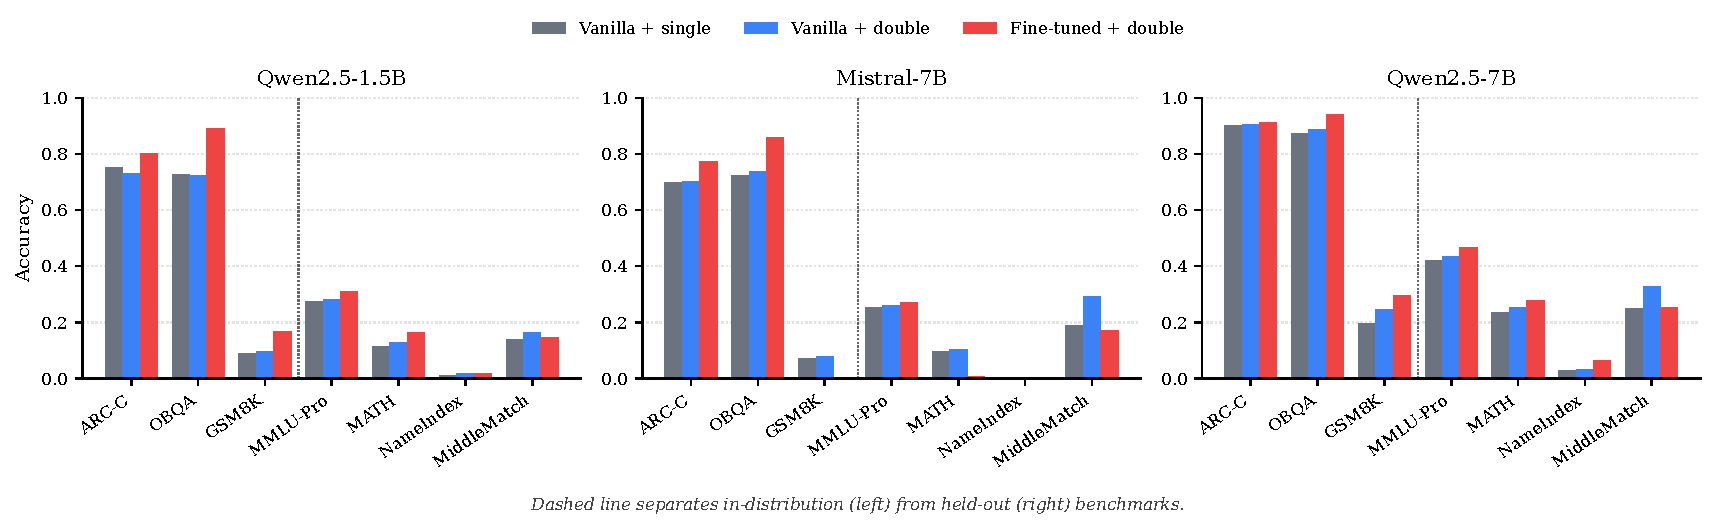
\includegraphics[width=\linewidth]{figures/main_results.pdf}
  \caption{Accuracy under the three conditions across all seven
  benchmarks and three base models. The dotted vertical line separates
  in-distribution (left) from held-out (right) benchmarks. Fine-tuning
  with doubled prompts (red) is almost always best or tied-best on the
  in-distribution benchmarks, but is not uniformly best on held-out
  tasks, and on Mistral-7B damages open-ended generation (GSM8K, MATH).}
  \label{fig:main}
\end{figure}

\begin{figure}[t]
  \centering
  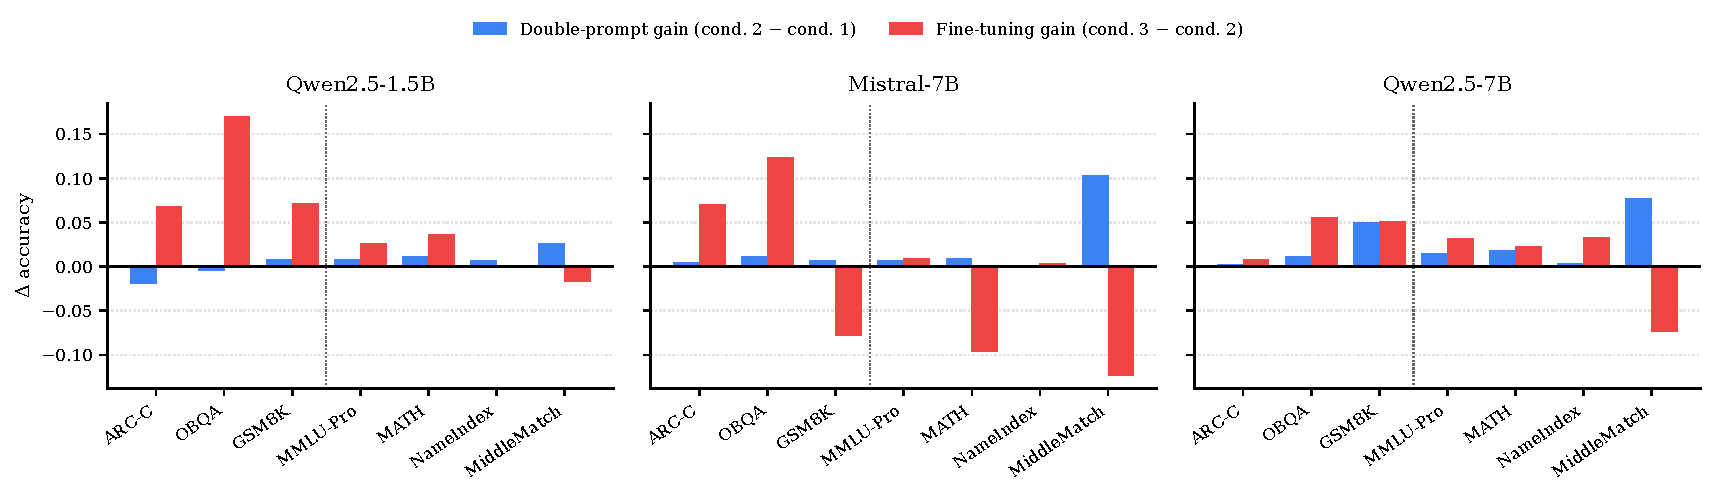
\includegraphics[width=\linewidth]{figures/gain_decomposition.pdf}
  \caption{Decomposition of accuracy changes. Blue: inference-time
  double-prompt gain, condition 2 $-$ condition 1. Red: additional gain
  from fine-tuning, condition 3 $-$ condition 2.}
  \label{fig:gain}
\end{figure}

\paragraph{Inference-time double prompting.}
The blue bars in \cref{fig:gain} show the pure inference-time effect.
Qwen2.5-7B and Mistral-7B show small but consistent gains (e.g.\
$+5.0$ pp on GSM8K for Qwen2.5-7B, $+1.5$ pp on MMLU-Pro) and large
gains on MiddleMatch ($+7.7$ and $+10.3$ pp), which matches the
intuition that repetition should help most when the relevant
information is long or positionally buried. Qwen2.5-1.5B, in contrast,
is essentially flat and mildly negative on the two multiple-choice
benchmarks---consistent with \citet{leviathan2025}'s observation that
the technique is less reliable on smaller models.

\paragraph{Training on doubled prompts.}
The red bars in \cref{fig:gain} are the main story.
On the three in-distribution benchmarks, fine-tuning helps every model
on every benchmark except Mistral-7B's GSM8K---and the gains are much
larger than the inference-time effect. Qwen2.5-1.5B gains $+17.0$ pp on
OpenBookQA, $+6.8$ pp on ARC, and $+7.1$ pp on GSM8K relative to its
already-doubled baseline; Qwen2.5-7B, despite a much higher starting
point, still gains $+5.6$, $+5.1$, and $+5.1$ pp. \Cref{fig:heat} shows
the total gain over the vanilla single-prompt baseline as a matrix: the
in-distribution columns are uniformly warm except for Mistral-7B's
GSM8K, and the held-out columns are much paler.

\begin{figure}[t]
  \centering
  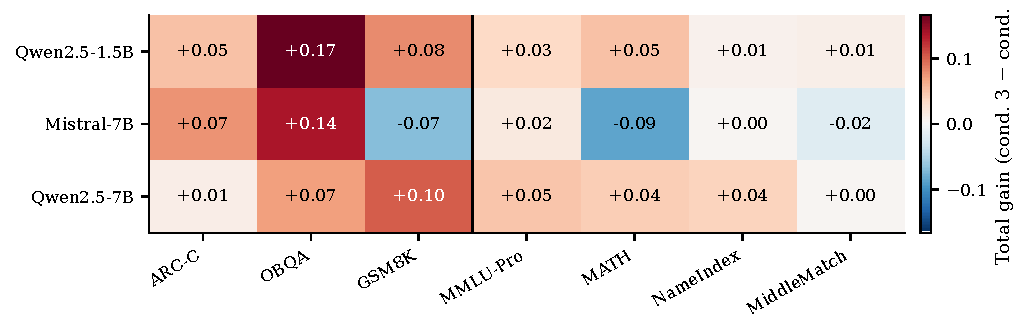
\includegraphics[width=0.95\linewidth]{figures/per_model_heatmap.pdf}
  \caption{Total gain of the fine-tuned double-prompt model over the
  vanilla single-prompt baseline, in accuracy. The solid vertical line
  separates in-distribution from held-out benchmarks.}
  \label{fig:heat}
\end{figure}

\paragraph{Held-out behaviour.}
The inference-time gain transfers roughly as well as it appears in
distribution---for Qwen2.5-7B and Mistral-7B the mean held-out
double-prompt gain ($+2.8$ and $+2.9$ pp) is actually larger than the
mean in-distribution gain, as one might hope from a generic
input-side intervention. The \emph{fine-tuning} gain does not
transfer cleanly. Held-out means are $+1.1$ pp for Qwen2.5-1.5B
(vs.\ $+10.4$ in-distribution), $+0.4$ for Qwen2.5-7B (vs.\ $+3.8$),
and a strongly negative $-5.2$ for Mistral-7B, driven by large drops on
MATH ($-9.6$) and MiddleMatch ($-12.3$).

\paragraph{Two failure modes.}
Two failures are worth calling out. First, Mistral-7B's fine-tuned
GSM8K accuracy collapses from $7.9\%$ to $0.08\%$, and MATH from
$10.3\%$ to $0.7\%$. Inspection of generations shows the fine-tuned
model reliably emits a single letter or short phrase even on
open-ended prompts---it has absorbed the multiple-choice output format
from ARC/OpenBookQA more strongly than the numeric format from GSM8K.
The Qwen family does not show the same collapse under the same data
mix, so this appears partly to be a Mistral-7B instruction-tuning
brittleness. Second, for both 7B models the inference-time double
prompt gives the single largest held-out gain on MiddleMatch ($+7.7$
and $+10.3$ pp)---exactly the sort of positional task the attention
story predicts---but fine-tuning then \emph{erases} that gain, pulling
the model back to roughly its single-prompt baseline. A plausible
reading is that the fine-tuned model's second-copy attention has been
specialized toward the in-distribution task formats and no longer
deploys the ``rescan the list'' behaviour that the vanilla base model
falls into on MiddleMatch.


\section{Discussion}

\paragraph{Take-away.}
Prompt repetition is \emph{learnable}: a model fine-tuned on doubled
prompts exploits the second copy substantially better than the vanilla
model on the kinds of tasks it was trained on. But the resulting skill
is local to the training distribution. It does not consistently add to
the transfer gains that inference-time repetition would have produced
on its own, and on structurally different tasks---or on brittle base
models with a biased training mix---it can actively hurt.

\paragraph{Strengths and weaknesses.}
The design cleanly separates the inference-time effect, the fine-tuning
effect, and their transfer behaviour, and running the same recipe on
three base models gives some confidence that the qualitative patterns
are not quirks of one checkpoint. The main weakness is a missing
control: we do not run \emph{single-prompt} fine-tuning with the same
data and compute, so part of what we attribute to doubling is simply
the gain from fine-tuning on these datasets at all. A clean ablation
would include a fourth condition, \emph{fine-tuned on single prompts},
evaluated under both single- and double-prompt inference.

\paragraph{Future work.}
The most natural next step is the missing ablation above. Beyond that,
it would be interesting to inspect whether the fine-tuned model's
second-copy attention patterns differ visibly from the base model's,
and to scale the training mix to something closer to a full
instruction-tuning corpus so that format-collapse failures like
Mistral-7B's are less likely to dominate.


\section{Conclusion}

Across three base models and seven benchmarks, training on doubled
prompts gives the largest accuracy gains we observe---but only in
distribution, and sometimes at the cost of open-ended generation.
Prompt repetition is best thought of as a cheap, format-level trick a
model can be taught to exploit, not as a universal way to improve
attention.




\printbibliography


%%%%%%%%%%%%%%%%%%%%%%%%%%%%%%%%%%%%%%%%%%%%%%%%%%%%%%%%%%%%

\appendix

\section{Full numerical results} \label{app:numbers}

\Cref{tab:qwen15,tab:mistral,tab:qwen7} give the raw accuracies
underlying \cref{fig:main,fig:gain,fig:heat}.
Columns $\Delta_{\text{DP}}$ and $\Delta_{\text{FT}}$ are the
double-prompt and fine-tuning gains respectively; $n$ is the number of
test examples evaluated.

\begin{table}[h]
  \caption{Qwen2.5-1.5B-Instruct.}
  \label{tab:qwen15}
  \centering
  \small
  \begin{tabular}{lrrrrrr}
    \toprule
    Benchmark      & $n$   & Single & Double & FT+Dbl & $\Delta_{\text{DP}}$ & $\Delta_{\text{FT}}$ \\
    \midrule
    ARC-Challenge  & 1172  & 0.752 & 0.732 & 0.800 & \neg{0.020} & \pos{0.068} \\
    OpenBookQA     & 500   & 0.726 & 0.722 & 0.892 & \neg{0.004} & \pos{0.170} \\
    GSM8K          & 1319  & 0.088 & 0.096 & 0.167 & \pos{0.008} & \pos{0.071} \\
    \midrule
    MMLU-Pro       & 2000  & 0.275 & 0.283 & 0.309 & \pos{0.008} & \pos{0.026} \\
    MATH           & 1000  & 0.115 & 0.127 & 0.163 & \pos{0.012} & \pos{0.036} \\
    NameIndex      & 300   & 0.010 & 0.017 & 0.017 & \pos{0.007} & $+0.000$ \\
    MiddleMatch    & 300   & 0.137 & 0.163 & 0.147 & \pos{0.027} & \neg{0.017} \\
    \bottomrule
  \end{tabular}
\end{table}

\begin{table}[h]
  \caption{Mistral-7B-Instruct.}
  \label{tab:mistral}
  \centering
  \small
  \begin{tabular}{lrrrrrr}
    \toprule
    Benchmark      & $n$   & Single & Double & FT+Dbl & $\Delta_{\text{DP}}$ & $\Delta_{\text{FT}}$ \\
    \midrule
    ARC-Challenge  & 1172  & 0.698 & 0.702 & 0.772 & \pos{0.004} & \pos{0.070} \\
    OpenBookQA     & 500   & 0.724 & 0.736 & 0.860 & \pos{0.012} & \pos{0.124} \\
    GSM8K          & 1319  & 0.072 & 0.079 & 0.001 & \pos{0.007} & \neg{0.078} \\
    \midrule
    MMLU-Pro       & 2000  & 0.254 & 0.260 & 0.270 & \pos{0.007} & \pos{0.010} \\
    MATH           & 1000  & 0.094 & 0.103 & 0.007 & \pos{0.009} & \neg{0.096} \\
    NameIndex      & 300   & 0.000 & 0.000 & 0.003 & $+0.000$    & \pos{0.003} \\
    MiddleMatch    & 300   & 0.190 & 0.293 & 0.170 & \pos{0.103} & \neg{0.123} \\
    \bottomrule
  \end{tabular}
\end{table}

\begin{table}[h]
  \caption{Qwen2.5-7B-Instruct.}
  \label{tab:qwen7}
  \centering
  \small
  \begin{tabular}{lrrrrrr}
    \toprule
    Benchmark      & $n$   & Single & Double & FT+Dbl & $\Delta_{\text{DP}}$ & $\Delta_{\text{FT}}$ \\
    \midrule
    ARC-Challenge  & 1172  & 0.903 & 0.905 & 0.914 & \pos{0.003} & \pos{0.009} \\
    OpenBookQA     & 500   & 0.874 & 0.886 & 0.942 & \pos{0.012} & \pos{0.056} \\
    GSM8K          & 1319  & 0.195 & 0.245 & 0.296 & \pos{0.050} & \pos{0.051} \\
    \midrule
    MMLU-Pro       & 2000  & 0.421 & 0.435 & 0.467 & \pos{0.015} & \pos{0.032} \\
    MATH           & 1000  & 0.236 & 0.254 & 0.277 & \pos{0.018} & \pos{0.023} \\
    NameIndex      & 300   & 0.027 & 0.030 & 0.063 & \pos{0.003} & \pos{0.033} \\
    MiddleMatch    & 300   & 0.250 & 0.327 & 0.253 & \pos{0.077} & \neg{0.073} \\
    \bottomrule
  \end{tabular}
\end{table}

\end{document}
